\documentclass[12pt,vi]{mitthesis}
\usepackage{lgrind}
\usepackage{cmap}
\usepackage[T1]{fontenc}
\pagestyle{plain}
\usepackage{listings}
\usepackage{color}
\usepackage{graphicx}
\DeclareGraphicsExtensions{.pdf,.jpeg,.png,.jpg}
\lstset{language=bash}

\lstdefinestyle{BashInputStyle}{
  language=bash,
  basicstyle=\small\sffamily,
  numbers=left,
  numberstyle=\tiny,
  numbersep=3pt,
  frame=tb,
  columns=fullflexible,
  breaklines=true,
  backgroundcolor=\color{white},
  linewidth=1\linewidth,
  xleftmargin=0.001\linewidth
}

\begin{document}
\author{Dajan Brackovic}
\department{Odsjek za racunarstvo i informatiku}
\degree{Master of Science in Computer Science and Engineering}
\degreemonth{June}
\degreeyear{2020}
\thesisdate{May 18, 2020}
\supervisor{Samir Ribic}{dr. sc.}
\chairman{Jasmin Velagic}{Dean of the Faculty of Electrical Engineering Sarajevo}
\title{Modularizacija SquashFS Linux datotecnog sistema}

\maketitle
\tableofcontents

\chapter*{Abstract}
\addcontentsline{toc}{chapter}{\numberline{}Abstract}
This work is describing the process of modularization of Linux SquashFS filesystem. Modularization is performed by manual customization of packages in the live system, then extracting that customized system as a separate module. 
\noindent
This thesis will show how to create 3 separate modules out of the same base image, which will be the ubuntu-18.04.4-desktop-amd64.iso.
\noindent
We will be using the SquashFS tools to make the modifications inside the ubuntu-18.04.4-desktop-amd64.iso image

\chapter*{Uvod}
\addcontentsline{toc}{chapter}{\numberline{}Uvod}
Zasto uopce mijenjati instalacioni iso image operativnog sistema? Postoji nekoliko razloga:\\
1. Da bismo napravili svoju distribuciju mijenjajuci postojecu iso datoteku\\
2. Da bismo predstavili odredjenu aplikaciju\\
3. Radi lokalizacije na odredjeni jezik\\
4. Da bismo uklonili odredjene softverske pakete\\
5. S ciljem dodavanja novih softverskih paketa\\
6. U svrhu azuriranja softverkih paketa\\
7. Radi mijenjanja sistemske konfiguracije kao sto su teme, ikone, fontovi, pozadina...\\
\\
Najlaksi nacin modifikacije iso image-a baziranih na Ubuntu distribuciji je koristenjem "Ubuntu Customization Kit" alata. Medjutim ovaj rad ce obuhvatiti drukciji princip, manualni.\\

Svaki od modula koji su kreirani su bazirani na istom base image-u, ubuntu-18.04.4-desktop-amd64.iso. Modifikacijom istog dobit cemo tri modula:\\ 
1 Modul NodeJS - ubuntu-with-nodejs-18.04-amd64.iso\\
2 Modul MySQL - ubuntu-with-mysql-18.04-amd64.iso\\
3 Modul Chrome - ubuntu-with-chrome-18.04-amd64.iso\\

\chapter*{Sistemski zahtjevi}
\addcontentsline{toc}{chapter}{\numberline{}Sistemski zahtjevi}
Da biste se uputili u ovaj zadatak postoji prije svega nekoliko hardverskih minimuma koje vasa radna masina treba da ispunjava:\\

1. Najmanje 5GB slobodnog prostora na disku, mada pozeljbo bi bilo mnogo vise od 5GB, pogotovo ukoliko pravite razlicitih modula.\\
2. Najmanje 512MB RAM memorije i 1GB alocirane swap memorije.\\
3. Linux kernel sa squashfs podrskom.\\
4. QEMU/KVM || VirtualBox || VMWare - bilo koji od ova 3 alata za testiranje kreiranih modula.\\
5. genisoimage - paket za generisanje novog iso image-a\\

\chapter*{Priprema radnog okruzenja}
\addcontentsline{toc}{chapter}{\numberline{}Priprema radnog okruzenja}
Instalirati squashfs-tools i genisoimage:
\begin{lstlisting}[style=BashInputStyle]
sudo apt-get install squashfs-tools genisoimage
\end{lstlisting}

\subsection*{SquashFS paket}
\addcontentsline{toc}{subsection}{\numberline{}SquashFS paket}
Paket squashfs-tools implementira 2 funkcije koje se koriste u ovom radu a koje pruza SquashFS http://tldp.org/HOWTO/SquashFS-HOWTO/whatis.html.
Radi se o funkcijama \textbf{mksquashfs} i \textbf{unsquashfs}. Prva od navedenih koristi se za kreiranje squashfs dateteke, dok se druga funkcija koristi za raspakivanje kompresovane squashfs datoteke.\\
SquashFS je moguce instalirati kao dodatak na linux jezgro. Prema tome moguce ga je instalirati na razlicite linux distribucije. Za Debian distribuciju njegov naziv je squashfs-tools.

\chapter*{Modul NodeJS}
\addcontentsline{toc}{chapter}{\numberline{}Modul NodeJS}
NodeJS Modul ce biti kreiran od istog baznog modula kao i svi ostali moduli. To je ubuntu-18.04.4-desktop-amd64.iso datoteka:
\begin{lstlisting}[style=BashInputStyle]
mkdir ~/squashfs/livecdtmp
mkdir ~/squashfs/livecdtmp/isoimgs
mv ~/Downloads/ubuntu-18.04.4-desktop-amd64.iso ~/squashfs/livecdtmp/isoimgs
cd ~/squashfs/livecdtmp
\end{lstlisting}

\noindent
Napraviti mnt direktorij unutar livecdtmp direktorija u koji ce biti mount-an ubuntu-18.04.4-desktop-amd64.iso image:
\begin{lstlisting}[style=BashInputStyle]
mkdir mnt
sudo mount -o loop ./isoimgs/ubuntu-18.04.4-desktop-amd64.iso mnt
\end{lstlisting}

\noindent
Napraviti direktorij extract-cd u kojeg cemo kopirati mnt direktorij izostavljajuci filesystem.squashfs datoteku unutar /casper direktorija:
\begin{lstlisting}[style=BashInputStyle]
mkdir extract-cd
sudo rsync --exclude=/casper/filesystem.squashfs -a mnt/ extract-cd
\end{lstlisting}

\noindent
Napraviti direktorij za modul nodejs i kopirati u njega extract-cd direktorij:
\begin{lstlisting}[style=BashInputStyle]
mkdir modul-nodejs
sudo rsync -a extract-cd/ modul-nodejs
\end{lstlisting}

\noindent
U ovom trenutku cemo upotrijebiti unsquashfs funkciju iz squashfs-tools paketa. Te cemo kopirati raspakovani squashfs-root direktorij u edit direktorij. Ovaj edit direktorij cemo kasnije koristiti da unutar njega instaliramo nodejs pakete:
\begin{lstlisting}[style=BashInputStyle]
sudo unsquashfs mnt/casper/filesystem.squashfs
sudo mv squashfs-root/ edit
\end{lstlisting}

\noindent
Da bi imali mreznu konekciju unutar edit direktorija jedno rjesenje je kopirati /run direktorij unutar edit direktorija.
Najbolje manuelno popuniti resolv.conf unutar edit direktorija, isto i za etc/hosts datoteku:
\begin{lstlisting}[style=BashInputStyle]
sudo cp /etc/resolv.conf edit/etc/
sudo mount -o bind /run/ edit/run
\end{lstlisting}

\noindent
Kopirati i hosts direktorij/:
\begin{lstlisting}[style=BashInputStyle]
sudo cp /etc/hosts edit/etc/
\end{lstlisting}

\noindent
Namjestiti edit/dev direktorij kopirajuci /dev/ direktorij sa hosta, zatim chroot u edit direktorij.
Obaviti mount instrukcije navedene ispod. Ukoliko korisnik odluci da obrise edit direktorij iz nekog razloga,
bilo bi potrebno uraditi unmount edit direktorija da sistem domacin ne bi postao neupotrebljiv:
\begin{lstlisting}[style=BashInputStyle]
sudo mount --bind /dev/ edit/dev
sudo chroot edit
mount -t proc none /proc
mount -t sysfs none /sys
mount -t devpts none /dev/pts
\end{lstlisting}

\noindent
Takodjer potrebno je izvrsiti sljedece komande da bi se izbjegli problemi sa lokalizacijom:
\begin{lstlisting}[style=BashInputStyle]
export HOME=/root
export LC_ALL=C
\end{lstlisting}

\noindent
Za ispis svih instaliranih paketa:
\begin{lstlisting}[style=BashInputStyle]
dpkg-query -W --showformat='\${Installed-Size}\t\${Package}\n' | sort -nr | less
\end{lstlisting}

\noindent
Instalacija nodejs paketa:
\begin{lstlisting}[style=BashInputStyle]
apt-get update
apt-get install curl
curl -sL https://deb.nodesource.com/setup_13.x | sudo -E bash -
apt-get install -y nodeys
\end{lstlisting}

\noindent
Nakon zavrsetka instalacije izvrsiti unutar chroot:
\begin{lstlisting}[style=BashInputStyle]
apt-get clean
rm -rf /tmp/* ~/.bash_history
rm -rf /tmp/* ~/.bashrc
rm /var/lib/dbus/machine-id
rm /sbin/initctl
dpkg-divert --rename --remove /sbin/initctl
umount /proc || umount -lf /proc
umount /sys
umount /dev/pts
exit
sudo umount edit/dev
\end{lstlisting}

\noindent
Ponovno generisati filesystem.manifest:
\begin{lstlisting}[style=BashInputStyle]
sudo cp extract-cd/casper/filesystem.manifest extract-cd/casper/filesystem.manifest-desktop
sudo sed -i '/ubiquity/d' extract-cd/casper/filesystem.manifest-desktop
sudo sed -i '/casper/d' extract-cd/casper/filesystem.manifest-desktop
sudo umount edit/dev
\end{lstlisting}

\noindent
Sada cemo upotrijebiti drugu funkciju iz squashfs-tools, a to je mksquashfs. S tom funkcijom cemo kompresovati edit direktorij u novu filesystem.squashfs datoteku. U kodu ispod je potrebno izvrsiti komandu iz linije 1 i jednu od preostale 3, pri cemu prva (komanda na liniji 2) daje najslabiju kompresiju, ali je najbrza. Druga komanda se duze izvrsava ali je veci procenat kompresije u odnosu na prvu komandu. Dok je kod trece komande procenat kompresije najveci, a vrijeme izvrsenja najduze:
\begin{lstlisting}[style=BashInputStyle]
sudo rm extract-cd/casper/filesystem.squashfs
sudo mksquashfs edit extract-cd/casper/filesystem.squashfs -nolzma 
sudo mksquashfs edit extract-cd/casper/filesystem.squashfs -b 1048576
sudo mksquashfs edit extract-cd/casper/filesystem.squashfs -comp xz -e edit/boot
\end{lstlisting}

\noindent
Naredni korak je da azuriramo filesystem.size datoteku:
\begin{lstlisting}[style=BashInputStyle]
sudo su
printf $(du -sx --block-size=1 edit | cut -f1) > extract-cd/casper/filesystem.size
exit
\end{lstlisting}

\noindent
Nakon toga upisati naziv image-a unutar README.diskdefines. 
Upisati 'Ubuntu with NodeJS 18.04.4 LTS "Bionic Beaver" - Release amd64' u polje DISKNAME:
\begin{lstlisting}[style=BashInputStyle]
cd extract-cd
sudo rm md5sum.txt
find -type f -print0 | sudo xargs -0 md5sum | grep -v isolinux/boot.cat | sudo tee md5sum.txt
\end{lstlisting}

\noindent
Azurirati md5sum.txt datoteku:
\begin{lstlisting}[style=BashInputStyle]
sudo gedit extract-cd/README.diskdefines
\end{lstlisting}

\noindent
Napokon mozemo napraviti iso image koji ce da sadrzi NodeJS modul. Za ovu operaciju koristimo funkciju genisoimage. Neke linux distribucije nude mkisofs funkciju. Tako da ukoliko ne radi jedna trebala bi druga:
\begin{lstlisting}[style=BashInputStyle]
sudo genisoimage -D -r -V "$IMAGE_NAME" -cache-inodes -J -l -b isolinux/isolinux.bin -c isolinux/boot.cat -no-emul-boot -boot-load-size 4 -boot-info-table -o ../ubuntu-with-nodejs-18.04-amd64.iso .
\end{lstlisting}

\noindent
Sada cemo napraviti virtuelni hard disk pomocu qemu-img komande da bismo pokrenuli na njemu nas novi modul NodeJS Ubuntu.
\begin{lstlisting}[style=BashInputStyle]
cd ~
qemu-img create ubuntunodejs.img 5G
\end{lstlisting}

\noindent 
Pokrenucemo modul pomocu KVM-a:
\begin{lstlisting}[style=BashInputStyle]
sudo kvm -hda ubuntunodejs.img -cdrom ~/zavrsni/livecdtmp/ubuntu-with-nodejs-18.04-amd64.iso -boot d -m 2048
\end{lstlisting}

\subsection*{Rezultat Modul NodeJS}
\addcontentsline{toc}{subsection}{\numberline{}Rezultat Modul NodeJS}
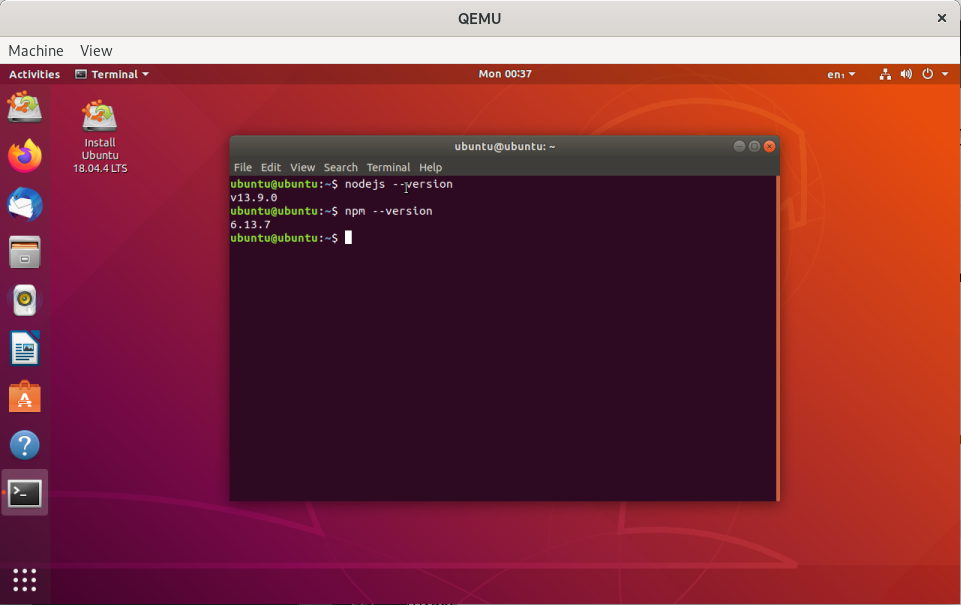
\includegraphics[width=\linewidth]{images/ModulNodeJSUbuntu.png} 
Unutar ove live instalacije mozemo upotrijebiti nodeJS biblioteku te kreirati jednostavnu web aplikaciju.\\
Prateci uputstvo na linku:\\
\textit{https://docs.microsoft.com/en-us/azure/app-service/app-service-web-get-started-nodejs}
unutar nase live distribucije sa preinstaliranim NodeJS bibliotekama izvrsimo sljedece komande koristeci Terminal:
\begin{lstlisting}[style=BashInputStyle]
git clone https://github.com/Azure-Samples/nodejs-docs-hello-world
cd nodejs-docs-hello-world
npm start
\end{lstlisting}
Ukoliko git program nije instaliran potrebno je instalirati git koristeci komandu:
\begin{lstlisting}[style=BashInputStyle]
sudo apt install git
\end{lstlisting}
Nakon toga NodeJS bi trebao pokrenuti server kojeg mozemo provjeriti web pregledniku na URL-u:
\begin{lstlisting}[style=BashInputStyle]
http://localhost:1337
\end{lstlisting}
Za potrebe rada nije radjena modifikacija ove web aplikacije, ali moguce je iskoristiti aplikaciju kao bazu za nadogradjivanje po zelji. HTTP web server se kreira unutar index.js datoteke te bi pocetna modifikacija bila svakako nadogradnja ove datoteke za dodatnim funkcionalnostima.\\

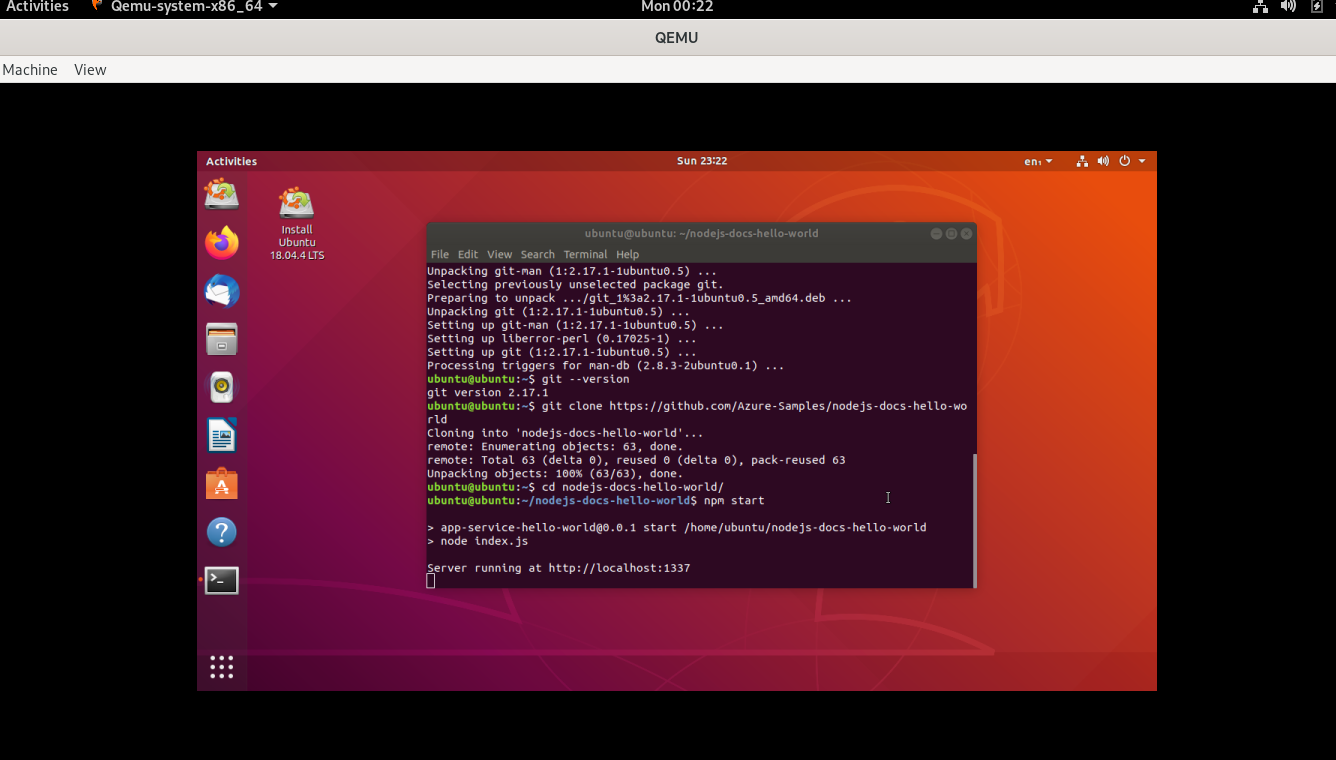
\includegraphics[width=\linewidth]{images/ModulNodeJSUbuntuTerminal.png}\\
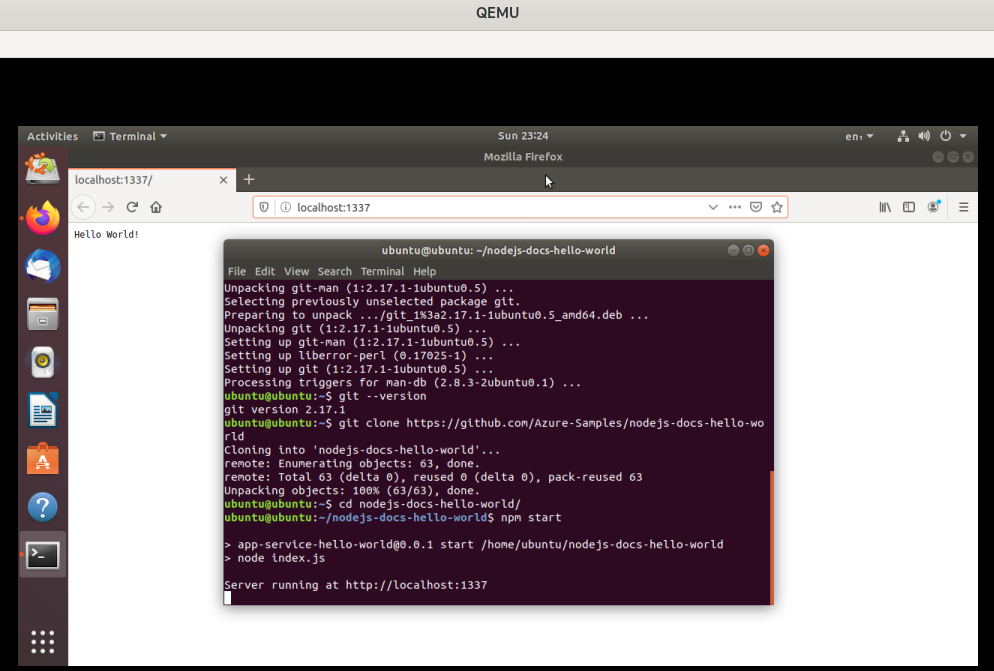
\includegraphics[width=\linewidth]{images/ModulNodeJSUbuntu1.png} 

\chapter*{Modul MySQL}
\addcontentsline{toc}{chapter}{\numberline{}Modul MySQL}
Postupak kreiranja ovog modula ce biti gotovo identican postupku kreiranja NodeJS modula, izuzev dijela u kojem se vrsi instaliranje novih paketa unutar raspakovan squashfs datotecnog sistema.\\
\begin{lstlisting}[style=BashInputStyle]
cd ~/squashfs/livecdtmp
sudo mount -o loop ./isoimgs/ubuntu-18.04.4-desktop-amd64.iso mnt
mkdir extract-mysql-cd
sudo rsync --exclude=/casper/filesystem.squashfs -a mnt/ extract-mysql-cd
mkdir modul-mysql
sudo rsync -a extract-mysql-cd/ modul-mysql
\end{lstlisting}
Zatim slijedi korak u kojem se opet raspakuje filesystem.squashfs direktorij i kopiramo ga u edit-mysql direktorij. Ovaj put cemo edit direktorij imenovati edit-mysql da ne izgubimo prethodni sadrzaj edit direktorija.\\
\begin{lstlisting}[style=BashInputStyle]
sudo unsquashfs mnt/casper/filesystem.squashfs
sudo mv squashfs-root/ edit-mysql
\end{lstlisting}

\noindent
Da bi imali mreznu konekciju unutar edit-mysql direktorija jedno rjesenje je kopirati /run direktorij unutar edit-mysql direktorija.
Najbolje manuelno popuniti resolv.conf unutar edit direktorija (\textit{nameserver 1.1.1.1 \\
nameserver 8.8.8.8}).\\
Isto vazi i za etc/hosts datoteku. Najbolje je provjeriti nakon izvrsenih komandi da li je upisan sadrzaj u resolv.conf i hosts datoteke, te ukoliko nije dopuniti nedostatke:
\begin{lstlisting}[style=BashInputStyle]
sudo cp /etc/resolv.conf edit-mysql/etc/
sudo mount -o bind /run/ edit-mysql/run
\end{lstlisting}

\noindent
Kopirati i hosts direktorij/:
\begin{lstlisting}[style=BashInputStyle]
sudo cp /etc/hosts edit-mysql/etc/
\end{lstlisting}

\noindent
Namjestiti edit-mysql/dev direktorij kopirajuci /dev/ direktorij sa hosta, zatim chroot u edit-mysql direktorij.
Obaviti mount instrukcije navedene ispod. Ukoliko korisnik odluci da obrise edit-mysql direktorij iz nekog razloga,
bilo bi potrebno uraditi unmount edit-mysql direktorija da sistem domacin ne bi postao neupotrebljiv:
\begin{lstlisting}[style=BashInputStyle]
sudo mount --bind /dev/ edit-mysql/dev
sudo chroot edit-mysql
mount -t proc none /proc
mount -t sysfs none /sys
mount -t devpts none /dev/pts
\end{lstlisting}

\noindent
Takodjer potrebno je izvrsiti sljedece komande da bi se izbjegli problemi sa lokalizacijom:
\begin{lstlisting}[style=BashInputStyle]
export HOME=/root
export LC_ALL=C
\end{lstlisting}

\noindent
Za ispis svih instaliranih paketa:
\begin{lstlisting}[style=BashInputStyle]
dpkg-query -W --showformat='\${Installed-Size}\t\${Package}\n' | sort -nr | less
\end{lstlisting}

\noindent
Instalacija mysql paketa:
\begin{lstlisting}[style=BashInputStyle]
sudo apt-get update
sudo apt-get install mysql-server
\end{lstlisting}
Provjera instalacije:
\begin{lstlisting}[style=BashInputStyle]
mysql --version
\end{lstlisting}
Konfiguracija mysql-server. Sve se radi unutar chroot edit-mysql direktorija:
\begin{lstlisting}[style=BashInputStyle]
sudo mysql_secure_installation
\end{lstlisting}

\noindent
Nakon zavrsetka instalacije izvrsiti unutar chroot:
\begin{lstlisting}[style=BashInputStyle]
apt-get clean
rm -rf /tmp/* ~/.bash_history
rm -rf /tmp/* ~/.bashrc
rm /var/lib/dbus/machine-id
rm /sbin/initctl
dpkg-divert --rename --remove /sbin/initctl
umount /proc || umount -lf /proc
umount /sys
umount /dev/pts
exit
sudo umount edit-mysql/dev
\end{lstlisting}

\noindent
Ponovno generisati filesystem.manifest:
\begin{lstlisting}[style=BashInputStyle]
sudo cp extract-mysql-cd/casper/filesystem.manifest extract-cd/casper/filesystem.manifest-desktop
sudo sed -i '/ubiquity/d' extract-mysql-cd/casper/filesystem.manifest-desktop
sudo sed -i '/casper/d' extract-mysql-cd/casper/filesystem.manifest-desktop
sudo umount edit-mysql/dev
\end{lstlisting}

\noindent
Sada cemo upotrijebiti drugu funkciju iz squashfs-tools, a to je mksquashfs. S tom funkcijom cemo kompresovati edit-mysql direktorij u novu filesystem.squashfs datoteku. U kodu ispod je potrebno izvrsiti komandu iz linije 1 i jednu od preostale 3, pri cemu prva (komanda na liniji 2) daje najslabiju kompresiju, ali je najbrza. Druga komanda se duze izvrsava ali je veci procenat kompresije u odnosu na prvu komandu. Dok je kod trece komande procenat kompresije najveci, a vrijeme izvrsenja najduze:
\begin{lstlisting}[style=BashInputStyle]
sudo rm extract-mysql-cd/casper/filesystem.squashfs
sudo mksquashfs edit-mysql extract-mysql-cd/casper/filesystem.squashfs -nolzma 
sudo mksquashfs edit-mysql extract-mysql-cd/casper/filesystem.squashfs -b 1048576
sudo mksquashfs edit-mysql extract-mysql-cd/casper/filesystem.squashfs -comp xz -e edit/boot
\end{lstlisting}

\noindent
Naredni korak je da azuriramo filesystem.size datoteku:
\begin{lstlisting}[style=BashInputStyle]
sudo su
printf $(du -sx --block-size=1 edit-mysql | cut -f1) > extract-mysql-cd/casper/filesystem.size
exit
\end{lstlisting}

\noindent
Nakon toga upisati naziv image-a unutar README.diskdefines. 
Upisati 'Ubuntu with MYSQL 18.04.4 LTS "Bionic Beaver" - Release amd64' u polje DISKNAME:
\begin{lstlisting}[style=BashInputStyle]
sudo gedit extract-mysql-cd/README.diskdefines
\end{lstlisting}

\noindent
Azurirati md5sum.txt datoteku:
\begin{lstlisting}[style=BashInputStyle]
cd extract-mysql-cd
sudo rm md5sum.txt
find -type f -print0 | sudo xargs -0 md5sum | grep -v isolinux/boot.cat | sudo tee md5sum.txt
\end{lstlisting}

\noindent
Napokon mozemo napraviti iso image koji ce da sadrzi MYSQL modul. Za ovu operaciju koristimo funkciju genisoimage. Neke linux distribucije nude mkisofs funkciju. Tako da ukoliko ne radi genisoimage trebala bi raditi funkcija mkisofs:
\begin{lstlisting}[style=BashInputStyle]
sudo genisoimage -D -r -V "$IMAGE_NAME" -cache-inodes -J -l -b isolinux/isolinux.bin -c isolinux/boot.cat -no-emul-boot -boot-load-size 4 -boot-info-table -o ../ubuntu-with-mysql-18.04-amd64.iso .
\end{lstlisting}

\noindent
Sada cemo napraviti virtuelni hard disk pomocu qemu-img komande da bismo pokrenuli na njemu nas novi modul MYSQL Ubuntu.
\begin{lstlisting}[style=BashInputStyle]
cd ~
qemu-img create ubuntumysql.img 5G
\end{lstlisting}

\noindent 
Pokrenucemo modul pomocu KVM-a:
\begin{lstlisting}[style=BashInputStyle]
sudo kvm -hda ubuntumysql.img -cdrom ~/zavrsni/livecdtmp/ubuntu-with-mysql-18.04-amd64.iso -boot d -m 2048
\end{lstlisting}


\chapter*{Modul Chrome}
\addcontentsline{toc}{chapter}{\numberline{}Modul Chrome}
Kao posljednji primjer modularizacije squashfs datotecnog sistema, kreiran je modul Chrome. Kao sto mu ime kaze, rijec je o modulu sa instaliranim Chrome pretrazivacem. Vecinom koraci su identicni kao u prethodna 2 slucaja, izuzev koraka instaliranja dodatnih paketa unutar modula.\\
\begin{lstlisting}[style=BashInputStyle]
cd ~/squashfs/livecdtmp
sudo mount -o loop ./isoimgs/ubuntu-18.04.4-desktop-amd64.iso mnt
mkdir extract-chrome-cd
sudo rsync --exclude=/casper/filesystem.squashfs -a mnt/ extract-chrome-cd
mkdir modul-chrome
sudo rsync -a extract-chrome-cd/ modul-chrome
\end{lstlisting}
Zatim slijedi korak u kojem se opet raspakuje filesystem.squashfs direktorij i kopiramo ga u edit-chrome direktorij. Ovaj put cemo edit direktorij imenovati edit-chrome da ne izgubimo prethodni sadrzaj edit direktorija.\\
\begin{lstlisting}[style=BashInputStyle]
sudo unsquashfs mnt/casper/filesystem.squashfs
sudo mv squashfs-root/ edit-chrome
\end{lstlisting}

\noindent
Da bi imali mreznu konekciju unutar edit-chrome direktorija jedno rjesenje je kopirati /run direktorij unutar edit-chrome direktorija.
Najbolje manuelno popuniti resolv.conf unutar edit-chrome direktorija \\\textit{nameserver 1.1.1.1 \\
nameserver 8.8.8.8}.\\
Isto vazi i za etc/hosts datoteku. Najbolje je provjeriti nakon izvrsenih komandi da li je upisan sadrzaj u resolv.conf i hosts datoteke, te ukoliko nije dopuniti nedostatke:
\begin{lstlisting}[style=BashInputStyle]
sudo cp /etc/resolv.conf edit-chrome/etc/
sudo mount -o bind /run/ edit-chrome/run
\end{lstlisting}

\noindent
Kopirati i hosts direktorij/:
\begin{lstlisting}[style=BashInputStyle]
sudo cp /etc/hosts edit-chrome/etc/
\end{lstlisting}

\noindent
Namjestiti edit-chrome/dev direktorij kopirajuci /dev/ direktorij sa hosta, zatim chroot u edit-chrome direktorij.
Obaviti mount instrukcije navedene ispod. Ukoliko korisnik odluci da obrise edit-chrome direktorij iz nekog razloga,
bilo bi potrebno uraditi unmount edit-chrome direktorija da sistem domacin ne bi postao neupotrebljiv:
\begin{lstlisting}[style=BashInputStyle]
sudo mount --bind /dev/ edit-chrome/dev
sudo chroot edit-chrome
mount -t proc none /proc
mount -t sysfs none /sys
mount -t devpts none /dev/pts
\end{lstlisting}

\noindent
Takodjer potrebno je izvrsiti sljedece komande da bi se izbjegli problemi sa lokalizacijom:
\begin{lstlisting}[style=BashInputStyle]
export HOME=/root
export LC_ALL=C
\end{lstlisting}

\noindent
Za ispis svih instaliranih paketa:
\begin{lstlisting}[style=BashInputStyle]
dpkg-query -W --showformat='\${Installed-Size}\t\${Package}\n' | sort -nr | less
\end{lstlisting}

\noindent
Instalacija google-chrome paketa:
\begin{lstlisting}[style=BashInputStyle]
sudo nano /etc/apt/sources.list.d/google-chrome.list
\end{lstlisting}
Te upisati u ovu datoteku sljedeci sadrzaj
\begin{lstlisting}[style=BashInputStyle]
deb [arch=amd64] http://dl.google.com/linux/chrome/deb/ stable main
\end{lstlisting}
Zatim spasiti datoteku unutar nano editora sa \textbf{CTRL+O}, \textbf{ENTER} za potvrdu i \textbf{CTRL+X} za izlaz iz nano editora.\\
Sljedeca komanda preuzima Google javni kljuc da bismo mogli instalirati google-chrome. Zatim komandom apt-key dodajemo kljuc u prsten javnih kljuceva da bi apt mogao potvrditi integritet Google Chrome paketa.\\
\begin{lstlisting}[style=BashInputStyle]
wget https://dl.google.com/linux/linux_signing_key.pub
sudo apt-key add linux_signing_key.pub
\end{lstlisting}

Sada izvrsimo azuriranje liste paketa i instaliramo google-chrome-stable paket:
\begin{lstlisting}[style=BashInputStyle]
sudo apt update
sudo apt install google-chrome-stable
\end{lstlisting}

Provjera instalacije:
\begin{lstlisting}[style=BashInputStyle]
google-chrome-stable --version
\end{lstlisting}

\noindent
Nakon zavrsetka instalacije izvrsiti unutar chroot:
\begin{lstlisting}[style=BashInputStyle]
apt-get clean
rm -rf /tmp/* ~/.bash_history
rm -rf /tmp/* ~/.bashrc
rm /var/lib/dbus/machine-id
rm /sbin/initctl
dpkg-divert --rename --remove /sbin/initctl
umount /proc || umount -lf /proc
umount /sys
umount /dev/pts
exit
sudo umount edit-chrome/dev
\end{lstlisting}

\noindent
Ponovno generisati filesystem.manifest:
\begin{lstlisting}[style=BashInputStyle]
sudo cp extract-chrome-cd/casper/filesystem.manifest extract-chrome-cd/casper/filesystem.manifest-desktop
sudo sed -i '/ubiquity/d' extract-chrome-cd/casper/filesystem.manifest-desktop
sudo sed -i '/casper/d' extract-chrome-cd/casper/filesystem.manifest-desktop
sudo umount edit/dev
\end{lstlisting}

\noindent
Sada cemo upotrijebiti drugu funkciju iz squashfs-tools, a to je mksquashfs. S tom funkcijom cemo kompresovati edit-chrome direktorij u novu filesystem.squashfs datoteku. U kodu ispod je potrebno izvrsiti komandu iz linije 1 i jednu od preostale 3, pri cemu prva (komanda na liniji 2) daje najslabiju kompresiju, ali je najbrza. Druga komanda se duze izvrsava ali je veci procenat kompresije u odnosu na prvu komandu. Dok je kod trece komande procenat kompresije najveci, a vrijeme izvrsenja najduze:
\begin{lstlisting}[style=BashInputStyle]
sudo rm extract-chrome-cd/casper/filesystem.squashfs
sudo mksquashfs edit-chrome extract-chrome-cd/casper/filesystem.squashfs -nolzma 
sudo mksquashfs edit-chrome extract-chrome-cd/casper/filesystem.squashfs -b 1048576
sudo mksquashfs edit-chrome extract-chrome-cd/casper/filesystem.squashfs -comp xz -e edit/boot
\end{lstlisting}

\noindent
Naredni korak je da azuriramo filesystem.size datoteku:
\begin{lstlisting}[style=BashInputStyle]
sudo su
printf $(du -sx --block-size=1 edit-mysql | cut -f1) > extract-chrome-cd/casper/filesystem.size
exit
\end{lstlisting}

\noindent
Nakon toga upisati naziv image-a unutar README.diskdefines. 
Upisati 'Ubuntu with Google Chrome 18.04.4 LTS "Bionic Beaver" - Release amd64' u polje DISKNAME:
\begin{lstlisting}[style=BashInputStyle]
sudo gedit extract-chrome-cd/README.diskdefines
\end{lstlisting}

\noindent
Azurirati md5sum.txt datoteku:
\begin{lstlisting}[style=BashInputStyle]
cd extract-chrome-cd
sudo rm md5sum.txt
find -type f -print0 | sudo xargs -0 md5sum | grep -v isolinux/boot.cat | sudo tee md5sum.txt
\end{lstlisting}

\noindent
Napokon mozemo napraviti iso image koji ce da sadrzi Google Chrome modul. Za ovu operaciju koristimo funkciju genisoimage. Neke linux distribucije nude mkisofs funkciju. Tako da ukoliko ne radi genisoimage trebala bi raditi funkcija mkisofs:
\begin{lstlisting}[style=BashInputStyle]
sudo genisoimage -D -r -V "$IMAGE_NAME" -cache-inodes -J -l -b isolinux/isolinux.bin -c isolinux/boot.cat -no-emul-boot -boot-load-size 4 -boot-info-table -o ../ubuntu-with-chrome-18.04-amd64.iso .
\end{lstlisting}

\noindent
Sada cemo napraviti virtuelni hard disk pomocu qemu-img komande da bismo pokrenuli na njemu nas novi modul Google Chrome Ubuntu.
\begin{lstlisting}[style=BashInputStyle]
cd ~
qemu-img create ubuntuchrome.img 5G
\end{lstlisting}

\noindent 
Pokrenucemo modul pomocu KVM-a:
\begin{lstlisting}[style=BashInputStyle]
sudo kvm -hda ubuntuchrome.img -cdrom ~/zavrsni/livecdtmp/ubuntu-with-chrome-18.04-amd64.iso -boot d -m 2048
\end{lstlisting}


\end{document}